% Drawing 69/05-7 -- folder 69, batch 05, archive page 86 (PDF page 87).
% Transcription: Une rangée de croquis : un segment pointé en son milieu ; un éventail de trois traits ; deux barres qui encadrent une croix ($|\times|$) ; trois barres parallèles ; deux barres et un triangle allongé ; une barre, une diagonale, une barre. Au-dessous, à gauche, un triangle et un éventail dont les sommets sont marqués $x$, $1$, $2$, $3$, $3'$, $4$, et un hexagone de sommets $\xi_3$, $\xi_{23}$, $\xi_2$, $\xi_{12}$, $\xi_1$, $\xi_{31}$, repassé, avec des cordes ; à côté, un pentagone.
% Kind: row of small sketches; triangle and fan; hexagon; pentagon. Method 2 (schematic redraw from the facsimile). Status: partial.
% Notes: A row of small sketches: a fan with a thick stroke, |x|, three parallel bars, two bars and an elongated triangle, a bar, a diagonal and a bar; below, a triangle and a fan (vertices x, 1, 2, 3, 3', 4, placed after the transcription), a hexagon xi_3, xi_23, xi_2, xi_12, xi_1, xi_31 inked over with inner chords, and a pentagon. The "segment pointed in its middle" is not identified with certainty (the short dotted stroke under the first fan). Approximate.
% Coordinates: 1 unit = 1 mm = 1/100 of the crop width (bbox in page fractions: [0.1, 0.3, 0.62, 0.48]).
% Redrawn by Claude (claude-opus-5-5), issue #73, 2026-11-07; not checked by a human; not compiled (no TeX in the session).
% Rights: reproduces part of the work -- behind RENDER_TRANSCRIPTS, never published by itself.
\documentclass[tikz,border=3pt]{standalone}
\usepackage{amsmath,amssymb}
\usetikzlibrary{patterns,arrows.meta}
\tikzset{pencil/.style={black!45}, struck/.style={black!35}, mark/.style={circle,draw,inner sep=1.3pt}, pt/.style={circle,fill,inner sep=0.9pt}, opt/.style={circle,draw,fill=white,inner sep=1.1pt}}
\begin{document}
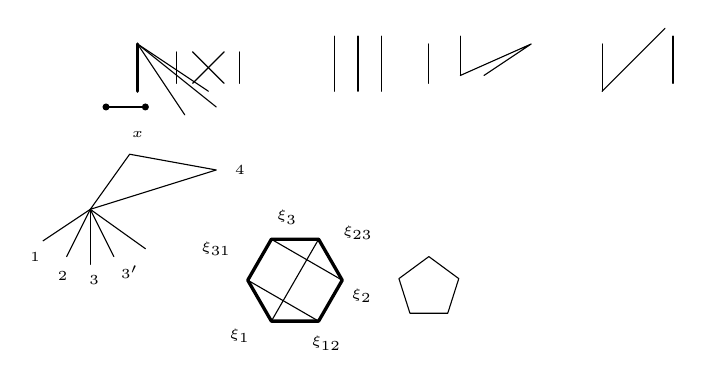
\begin{tikzpicture}[x=1mm,y=1mm,line cap=round,line join=round,font=\scriptsize]
\draw[very thick] (24,-4) -- (24,-10);
\draw (24,-4) -- (34,-12);
\draw (24,-4) -- (33,-10);
\draw (24,-4) -- (30,-13);
\draw (20,-12) -- (25,-12);
\node[pt] at (20,-12) {};
\node[pt] at (25,-12) {};
\draw (29,-5) -- (29,-9);
\draw (37,-5) -- (37,-9);
\draw (31,-5) -- (35,-9);
\draw (35,-5) -- (31,-9);
\draw (49,-3) -- (49,-10);
\draw (52,-3) -- (52,-10);
\draw (55,-3) -- (55,-10);
\draw (61,-4) -- (61,-9);
\draw (65,-3) -- (65,-8);
\draw (65,-8) -- (74,-4) -- (68,-8);
\draw (83,-4) -- (83,-10);
\draw (83,-10) -- (91,-2);
\draw (92,-3) -- (92,-9);
\draw (18,-25) -- (23,-18) -- (34,-20) -- cycle;
\draw (18,-25) -- (12,-29);
\draw (18,-25) -- (15,-31);
\draw (18,-25) -- (18,-32);
\draw (18,-25) -- (21,-31);
\draw (18,-25) -- (25,-30);
\node[inner sep=1pt] at (24,-15.5) {\tiny $x$};
\node[inner sep=1pt] at (37,-20) {\tiny $4$};
\node[inner sep=1pt] at (11,-31) {\tiny $1$};
\node[inner sep=1pt] at (14.5,-33.5) {\tiny $2$};
\node[inner sep=1pt] at (18.5,-34) {\tiny $3$};
\node[inner sep=1pt] at (23,-33) {\tiny $3'$};
\draw[very thick] (50,-34) -- (47,-28.8) -- (41,-28.8) -- (38,-34) -- (41,-39.2) -- (47,-39.2) -- cycle;
\draw (50,-34) -- (41,-28.8);
\draw (38,-34) -- (47,-39.2);
\draw (47,-28.8) -- (41,-39.2);
\node[inner sep=1pt] at (43,-26) {\tiny $\xi_3$};
\node[inner sep=1pt] at (52,-28) {\tiny $\xi_{23}$};
\node[inner sep=1pt] at (52.5,-36) {\tiny $\xi_2$};
\node[inner sep=1pt] at (48,-42) {\tiny $\xi_{12}$};
\node[inner sep=1pt] at (37,-41) {\tiny $\xi_1$};
\node[inner sep=1pt] at (34,-30) {\tiny $\xi_{31}$};
\draw (61,-31) -- (57.2,-33.8) -- (58.6,-38.2) -- (63.4,-38.2) -- (64.8,-33.8) -- cycle;
\end{tikzpicture}
\end{document}
